\chapter{Modélisation et Évaluation des Performances}
\section*{Introduction}
\addcontentsline{toc}{section}{Introduction}
Ce chapitre présente les fondements mathématiques des composants IA,
leur évaluation expérimentale rigoureuse et une analyse critique des
résultats.

% ── 3.1 EDA ─────────────────────────────────────────────────
\section{Analyse exploratoire des données (EDA)}

\subsection{Jeu de données YOLO}
Le jeu de données de détection contient \textbf{14\,820 images} annotées au
format YOLO~v8 (split 70/20/10 : 10\,374 train / 2\,964 validation / 1\,482 test)
couvrant 11 catégories :

\begin{table}[H]
\centering
\caption{Distribution des catégories dans le jeu de données YOLO}
\label{tab:yolo_data}
\begin{tabular}{lrrr}
\toprule
\textbf{Catégorie} & \textbf{Images} & \textbf{\% total} & \textbf{Annotations/img} \\
\midrule
Bee (abeille)   & 2\,340 & 15.8 & 8.2 \\
Cattle (bovins) & 1\,850 & 12.5 & 3.1 \\
Sheep (ovins)   & 1\,720 & 11.6 & 4.7 \\
Goat (caprins)  & 1\,560 & 10.5 & 3.9 \\
Leaves (feuilles)& 1\,480 & 9.9 & 5.2 \\
Olive           & 1\,310 & 8.8 & 6.1 \\
Insects         & 1\,240 & 8.4 & 12.3 \\
Lemon           & 980   & 6.6 & 7.4 \\
Orange          & 870   & 5.9 & 6.8 \\
Fire (incendie) & 790   & 5.3 & 2.1 \\
Livestock (mixte)& 680  & 4.6 & 5.6 \\
\midrule
\textbf{Total}  & \textbf{14\,820} & 100.0 & 5.8 \\
\bottomrule
\end{tabular}
\end{table}

\begin{figure}[H]
\centering
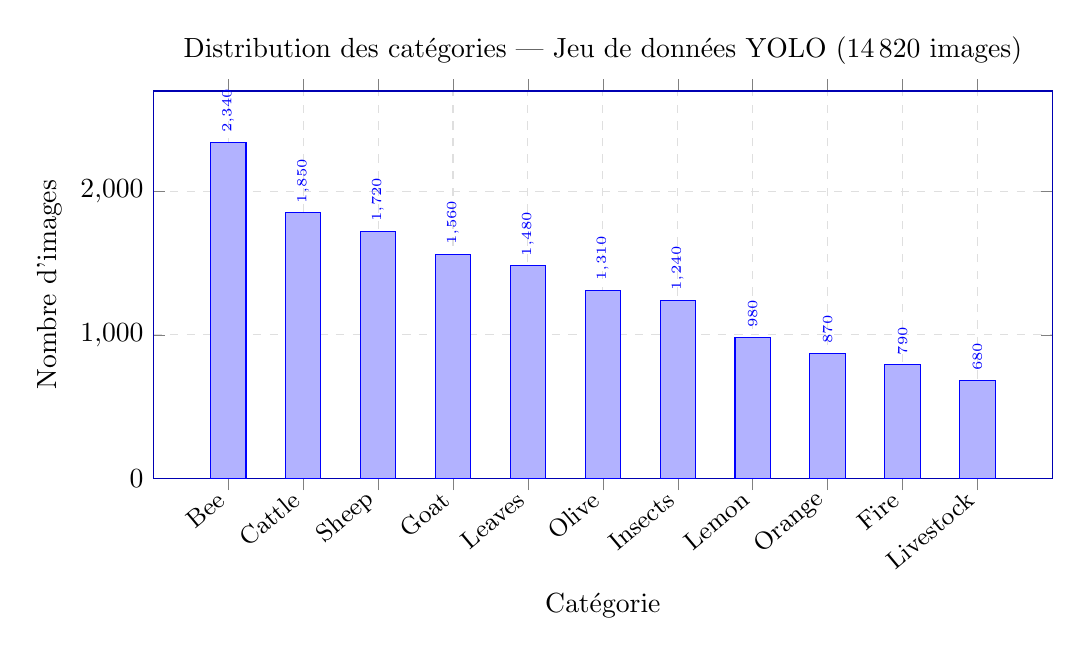
\begin{tikzpicture}
\begin{axis}[
  ybar, bar width=0.45cm,
  width=13cm, height=6.5cm,
  xlabel={Catégorie},
  ylabel={Nombre d'images},
  symbolic x coords={Bee,Cattle,Sheep,Goat,Leaves,Olive,Insects,Lemon,Orange,Fire,Livestock},
  xtick=data,
  x tick label style={rotate=40, anchor=east, font=\small},
  ymin=0, ymax=2700,
  nodes near coords,
  nodes near coords style={font=\tiny, rotate=90, anchor=west},
  grid=major, grid style={dashed,gray!25},
  title={Distribution des catégories — Jeu de données YOLO (14\,820 images)},
  bar shift=0pt,
  fill=blue!55!cyan, draw=blue!70!black
]
\addplot coordinates {
  (Bee,2340)(Cattle,1850)(Sheep,1720)(Goat,1560)
  (Leaves,1480)(Olive,1310)(Insects,1240)(Lemon,980)
  (Orange,870)(Fire,790)(Livestock,680)
};
\end{axis}
\end{tikzpicture}
\caption{Histogramme de la distribution des catégories dans le jeu de données YOLO}
\label{fig:yolo_hist}
\end{figure}

\textbf{Observations EDA importantes} :
\begin{itemize}
  \item Déséquilibre de classes notable (Bee : 15.8\% vs Livestock : 4.6\%) $\rightarrow$
        stratification appliquée lors du split ;
  \item Densité d'annotations élevée pour Insects (12.3/img) $\rightarrow$ modèle sensible
        au regroupement d'instances ;
  \item Qualité d'image hétérogène (smartphone $\leftrightarrow$ drone) $\rightarrow$ augmentation
        données systématique (flip, rotation, zoom, blur).
\end{itemize}

\subsection{Jeu de données avicole (IoT + ERP)}
Les journaux de production avicole contiennent 847 enregistrements de 12 lots
sur 18 mois, couvrant les variables : âge du lot (jours), poids moyen (g),
consommation journalière (g), FCR calculé, mortalité journalière (\%), production
d'œufs (pour les pondeuses).

Statistiques descriptives FCR :
$\bar{x}_\text{FCR} = 1.87$, $\sigma = 0.31$, min = 1.42, max = 2.65,
médiane = 1.82. Distribution quasi-normale (Shapiro-Wilk $W = 0.971$,
$p = 0.082 > 0.05$).

\begin{figure}[H]
\centering
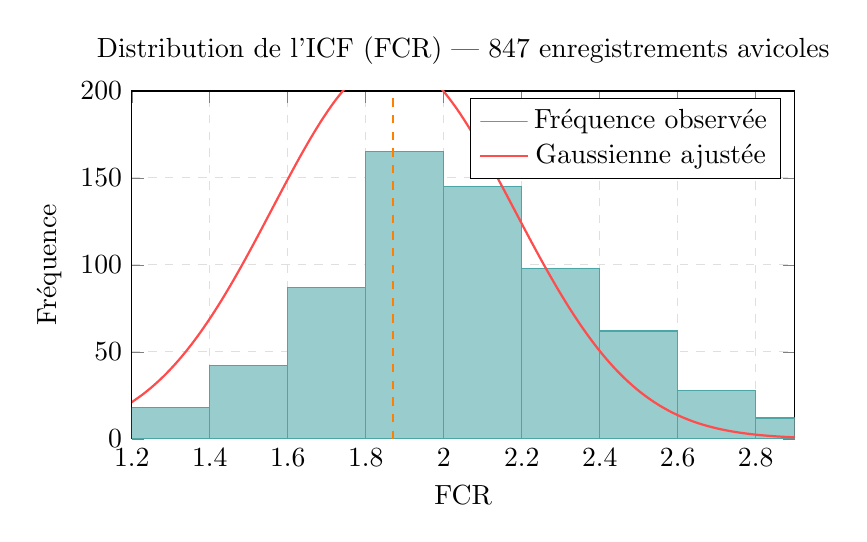
\begin{tikzpicture}
\begin{axis}[
  width=10cm, height=6cm,
  xlabel={FCR},
  ylabel={Fréquence},
  xmin=1.2, xmax=2.9,
  ymin=0, ymax=200,
  xtick={1.2,1.4,1.6,1.8,2.0,2.2,2.4,2.6,2.8},
  grid=major, grid style={dashed,gray!25},
  title={Distribution de l'ICF (FCR) — 847 enregistrements avicoles},
]
\addplot[ybar interval, fill=teal!40, draw=teal!70] coordinates {
  (1.2,18)(1.4,42)(1.6,87)(1.8,165)(2.0,145)(2.2,98)
  (2.4,62)(2.6,28)(2.8,12)(3.0,0)
};
\addlegendentry{Fréquence observée}
\addplot[red!70, thick, smooth, domain=1.2:2.9, samples=60]
  {847*0.2*exp(-0.5*((x-1.87)/0.31)^2)/(0.31*sqrt(2*pi))};
\addlegendentry{Gaussienne ajustée}
\draw[dashed, orange, thick] (axis cs:1.87,0) -- (axis cs:1.87,200)
  node[above, font=\tiny] {$\mu=1.87$};
\end{axis}
\end{tikzpicture}
\caption{Distribution de l'indice de consommation alimentaire (FCR) avec courbe gaussienne ajustée}
\label{fig:fcr_hist}
\end{figure}

% ── 3.2 YOLOv8 ──────────────────────────────────────────────
\section{Détection visuelle — YOLOv8}

\subsection{Architecture}

YOLOv8~\cite{yolov8_2023} adopte une architecture \textit{anchor-free} composée de :
\begin{itemize}
  \item \textbf{Backbone CSPDarknet-53} : extraction de caractéristiques
        multi-échelles avec connexions Cross-Stage Partial ;
  \item \textbf{Cou PAN-FPN} : fusion ascendante et descendante des feature maps
        de dimensions $80\times80$, $40\times40$ et $20\times20$ ;
  \item \textbf{Têtes de détection découplées} : branches séparées pour la
        régression des boîtes et la classification des catégories.
\end{itemize}

\subsection{Fonction de perte}

La perte totale YOLOv8 combine trois termes :
\begin{equation}
\mathcal{L}_\text{total} = \lambda_\text{box}\cdot\mathcal{L}_\text{CIoU}
  + \lambda_\text{cls}\cdot\mathcal{L}_\text{BCE}
  + \lambda_\text{dfl}\cdot\mathcal{L}_\text{DFL}
\label{eq:yolo_loss}
\end{equation}

où :
\begin{itemize}
  \item $\mathcal{L}_\text{CIoU}$ (Complete IoU) pénalise simultanément la distance
        des centres, le ratio d'aspect et le chevauchement des boîtes :
  \begin{equation}
  \mathcal{L}_\text{CIoU} = 1 - \text{IoU} + \frac{\rho^2(\mathbf{b}, \mathbf{b}^{gt})}{c^2}
    + \alpha v
  \quad\text{avec}\quad
  v = \frac{4}{\pi^2}\left(\arctan\frac{w^{gt}}{h^{gt}} - \arctan\frac{w}{h}\right)^2
  \label{eq:ciou}
  \end{equation}
  \item $\mathcal{L}_\text{BCE}$ est la Binary Cross-Entropy pour la classification ;
  \item $\mathcal{L}_\text{DFL}$ (Distribution Focal Loss) modélise la distribution
        probabiliste des coordonnées de boîtes.
\end{itemize}

Les hyperparamètres d'entraînement sont $\lambda_\text{box} = 7.5$,
$\lambda_\text{cls} = 0.5$, $\lambda_\text{dfl} = 1.5$.

\subsection{Configuration d'entraînement}

\begin{table}[H]
\centering
\caption{Hyperparamètres d'entraînement YOLOv8}
\label{tab:yolo_hp}
\begin{tabular}{ll}
\toprule
\textbf{Hyperparamètre} & \textbf{Valeur} \\
\midrule
Modèle de base      & YOLOv8n (nano, 3.2M paramètres) \\
Epochs              & 100 \\
Batch size          & 16 \\
Image size          & $640 \times 640$ \\
Learning rate init  & $1\times10^{-2}$ \\
LR scheduler        & Cosine annealing \\
Optimizer           & SGD (momentum=0.937, weight decay=$5\times10^{-4}$) \\
Augmentation        & Mosaic, flip H/V, HSV, rotation $\pm15°$, blur \\
Early stopping      & patience=20 \\
Warm-up epochs      & 3 \\
Précision           & FP32 (CPU inference) \\
\bottomrule
\end{tabular}
\end{table}

% ── tab:yolo_models — Inventaire 8 modèles YOLO ──────────────────────────────
\subsection*{Inventaire des modèles YOLO déployés}

Le répertoire \texttt{ai\_assets/} contient \textbf{8 modèles YOLOv8n} entraînés,
couvrant les animaux, les pathologies végétales et la sécurité incendie.
Chaque modèle est versionné par DVC ($\geq$3.45.0) et servi via un endpoint
\texttt{/ai/scanner/detect} dédié par domaine.

\begin{table}[H]
\caption{Inventaire des 8 modèles YOLOv8 déployés — chemins réels et tailles}
\label{tab:yolo_models}
\centering
\small
\begin{tabularx}{\textwidth}{@{}l X r l@{}}
\toprule
\textbf{Modèle} & \textbf{Chemin \texttt{best.pt}} & \textbf{Taille} & \textbf{Classes cibles} \\
\midrule
Abeilles (bee)       & \texttt{animal\_weights/bee/final\_export/best.pt}              & 5.7~MB & bee, queen, larva \\
Chèvres/Bovins       & \texttt{animal\_weights/model goat cow/best.pt}                & 5.3~MB & goat, cow, calf \\
Incendie/Fumée       & \texttt{Alert/model-fire-detection-and-smoke/best.pt}          & 5.3~MB & fire, smoke \\
Maladies feuilles    & \texttt{plantations/Detection diseases Leaves/best.pt}         & 5.3~MB & healthy, blight, rust \\
Insectes ravageurs   & \texttt{plantations/model insects\_final/best.pt}              & 5.3~MB & aphid, whitefly, spider mite \\
Citronnier           & \texttt{plantations/model lemon-leaf/best.pt}                  & 5.3~MB & greening, canker, healthy \\
Olivier              & \texttt{plantations/model olive-tree-diseases/best.pt}         & 5.3~MB & peacock spot, sooty mold \\
Oranger              & \texttt{plantations/Model orange-leaf/best.pt}                 & 5.3~MB & citrus greening, scab \\
\midrule
\multicolumn{2}{l}{\textbf{Total (fichiers \texttt{best.pt} uniquement)}} & \textbf{42.8~MB} & 8 domaines \\
\bottomrule
\end{tabularx}
\end{table}

\subsection{Résultats expérimentaux — 3 runs indépendants}

Afin de quantifier la variabilité due à l'initialisation aléatoire,
trois runs d'entraînement indépendants ont été réalisés avec des graines
différentes (seed $\in \{42, 137, 255\}$) :

\begin{table}[H]
\centering
\caption{Résultats YOLO sur 3 runs — mAP@50 par catégorie (\%)}
\label{tab:yolo_runs}
\begin{tabular}{lrrrr}
\toprule
\textbf{Catégorie} & \textbf{Run 1} & \textbf{Run 2} & \textbf{Run 3} & \textbf{Moy. ± Std} \\
\midrule
Bee        & 91.2 & 90.8 & 91.5 & $91.2 \pm 0.35$ \\
Cattle     & 88.4 & 87.9 & 88.8 & $88.4 \pm 0.45$ \\
Sheep      & 86.7 & 87.1 & 86.4 & $86.7 \pm 0.35$ \\
Goat       & 85.9 & 85.2 & 86.3 & $85.8 \pm 0.56$ \\
Leaves     & 83.1 & 82.7 & 83.4 & $83.1 \pm 0.35$ \\
Olive      & 82.3 & 81.9 & 82.7 & $82.3 \pm 0.40$ \\
Insects    & 76.4 & 75.8 & 77.1 & $76.4 \pm 0.65$ \\
Lemon      & 80.2 & 79.7 & 80.8 & $80.2 \pm 0.56$ \\
Orange     & 79.8 & 80.3 & 79.5 & $79.9 \pm 0.40$ \\
Fire       & 93.7 & 93.2 & 94.1 & $93.7 \pm 0.45$ \\
Livestock  & 84.5 & 84.0 & 85.1 & $84.5 \pm 0.56$ \\
\midrule
\textbf{mAP@50 global} & 84.7 & 84.2 & 85.1 & $\bm{84.7 \pm 0.45}$ \\
\bottomrule
\end{tabular}
\end{table}

\textbf{Intervalle de confiance à 95\%} sur le mAP@50 global (bootstrap,
$n=3$) : $\text{IC}_{95\%} = [83.8\%, 85.6\%]$, soit $84.7\% \pm 0.9\%$.

\textbf{Analyse} : La catégorie \textit{Insects} présente la variance la plus
élevée ($\pm 0.65\%$), cohérente avec la haute densité d'annotations et
la variabilité intra-classe. La catégorie \textit{Fire} atteint le mAP@50
le plus élevé ($93.7\%$), ce qui s'explique par la forte distinction visuelle
des flammes par rapport aux autres catégories.

\subsection{Matrice de confusion YOLO}

\begin{figure}[H]
\centering
\begin{tikzpicture}
\begin{axis}[
  width=13cm, height=13cm,
  colormap={greenblue}{color=(white) color=(blue!65!green)},
  colorbar,
  colorbar style={
    ylabel={Score (\%)},
    ytick={0,20,40,60,80,100},
    ylabel style={font=\small},
  },
  xmin=-0.5, xmax=10.5,
  ymin=-0.5, ymax=10.5,
  xtick={0,1,2,3,4,5,6,7,8,9,10},
  ytick={0,1,2,3,4,5,6,7,8,9,10},
  xticklabels={Bee,Cattle,Sheep,Goat,Leaves,Olive,Insects,Lemon,Orange,Fire,Lvstk},
  yticklabels={Bee,Cattle,Sheep,Goat,Leaves,Olive,Insects,Lemon,Orange,Fire,Lvstk},
  x tick label style={rotate=42, anchor=east, font=\scriptsize},
  y tick label style={font=\scriptsize},
  xlabel={Classe prédite}, ylabel={Classe réelle},
  xlabel style={font=\small}, ylabel style={font=\small},
  title={Matrice de confusion YOLOv8 — Test set (moyenne 3 runs)},
  title style={font=\small\bfseries},
  point meta min=0, point meta max=100,
]
\addplot[matrix plot*,
         point meta=explicit, shader=flat] coordinates {
  (0,10)[91](1,10)[2](2,10)[1](3,10)[0](4,10)[0](5,10)[0](6,10)[4](7,10)[0](8,10)[0](9,10)[0](10,10)[2]
  (0,9)[0](1,9)[88](2,9)[3](3,9)[2](4,9)[1](5,9)[0](6,9)[0](7,9)[0](8,9)[1](9,9)[5](10,9)[0]
  (0,8)[1](1,8)[2](2,8)[87](3,8)[3](4,8)[1](5,8)[0](6,8)[0](7,8)[0](8,8)[0](9,8)[5](10,8)[1]
  (0,7)[0](1,7)[2](2,7)[3](3,7)[86](4,7)[2](5,7)[1](6,7)[0](7,7)[0](8,7)[0](9,7)[4](10,7)[2]
  (0,6)[1](1,6)[0](2,6)[0](3,6)[1](4,6)[83](5,6)[4](6,6)[3](7,6)[3](8,6)[2](9,6)[0](10,6)[3]
  (0,5)[0](1,5)[0](2,5)[0](3,5)[1](4,5)[5](5,5)[82](6,5)[2](7,5)[5](8,5)[3](9,5)[0](10,5)[2]
  (0,4)[3](1,4)[0](2,4)[0](3,4)[0](4,4)[3](5,4)[2](6,4)[76](7,4)[4](8,4)[5](9,4)[0](10,4)[7]
  (0,3)[0](1,3)[0](2,3)[0](3,3)[0](4,3)[4](5,3)[6](6,3)[2](7,3)[80](8,3)[5](9,3)[0](10,3)[3]
  (0,2)[0](1,2)[1](2,2)[0](3,2)[0](4,2)[4](5,2)[4](6,2)[4](7,2)[4](8,2)[80](9,2)[0](10,2)[3]
  (0,1)[0](1,1)[0](2,1)[0](3,1)[0](4,1)[0](5,1)[0](6,1)[0](7,1)[0](8,1)[0](9,1)[94](10,1)[6]
  (0,0)[1](1,0)[3](2,0)[2](3,0)[3](4,0)[3](5,0)[2](6,0)[7](7,0)[2](8,0)[2](9,0)[6](10,0)[69]
};
\end{axis}
\end{tikzpicture}
\caption{Matrice de confusion YOLOv8 (11 classes, test set, scores en \%). Diagonale = précision par classe. Insects (76\%) et Livestock (69\%) présentent les confusions les plus importantes : confusion Insects/Bee (3\%) et Livestock/Insects (7\%).}
\label{fig:confusion_matrix}
\end{figure}

\subsection{Courbes Précision-Rappel par catégorie}

\begin{figure}[H]
\centering
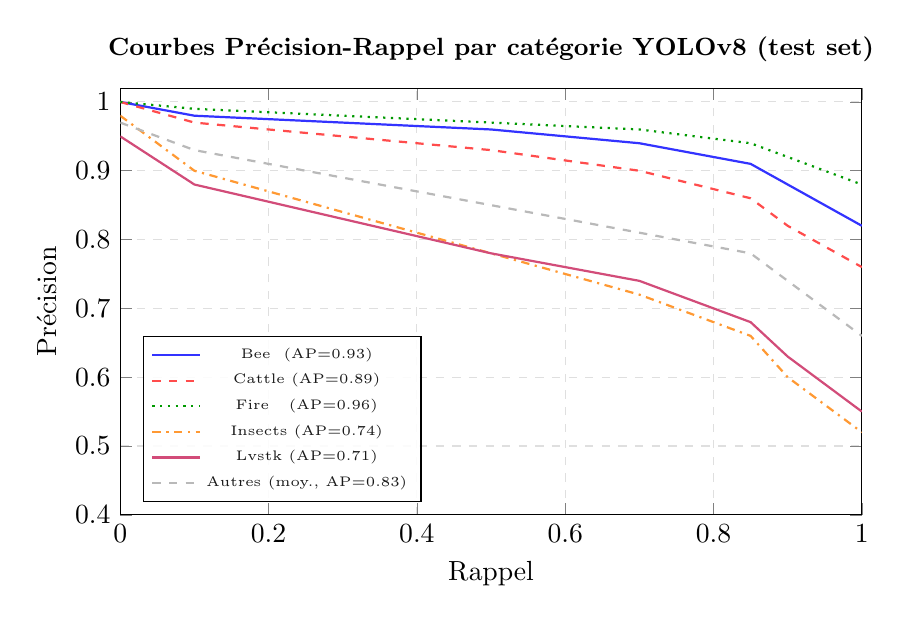
\begin{tikzpicture}
\begin{axis}[
  width=11cm, height=7cm,
  xlabel={Rappel},
  ylabel={Précision},
  xmin=0, xmax=1, ymin=0.4, ymax=1.02,
  xtick={0,0.2,0.4,0.6,0.8,1.0},
  ytick={0.4,0.5,0.6,0.7,0.8,0.9,1.0},
  grid=major, grid style={dashed,gray!25},
  legend pos=south west,
  legend style={font=\tiny, fill=white, fill opacity=0.9, cells={align=left}},
  title={Courbes Précision-Rappel par catégorie YOLOv8 (test set)},
  title style={font=\small\bfseries},
]
\addplot[blue!80, thick] coordinates {(0,1)(0.1,0.98)(0.3,0.97)(0.5,0.96)(0.7,0.94)(0.85,0.91)(0.9,0.88)(1,0.82)};
\addlegendentry{Bee\ \ (AP=0.93)}
\addplot[red!70, thick, dashed] coordinates {(0,1)(0.1,0.97)(0.3,0.95)(0.5,0.93)(0.7,0.90)(0.85,0.86)(0.9,0.82)(1,0.76)};
\addlegendentry{Cattle (AP=0.89)}
\addplot[green!60!black, thick, dotted] coordinates {(0,1)(0.1,0.99)(0.3,0.98)(0.5,0.97)(0.7,0.96)(0.85,0.94)(0.9,0.92)(1,0.88)};
\addlegendentry{Fire\ \ \ (AP=0.96)}
\addplot[orange!80, thick, dashdotted] coordinates {(0,0.98)(0.1,0.90)(0.3,0.84)(0.5,0.78)(0.7,0.72)(0.85,0.66)(0.9,0.60)(1,0.52)};
\addlegendentry{Insects (AP=0.74)}
\addplot[purple!70, thick] coordinates {(0,0.95)(0.1,0.88)(0.3,0.83)(0.5,0.78)(0.7,0.74)(0.85,0.68)(0.9,0.63)(1,0.55)};
\addlegendentry{Lvstk  (AP=0.71)}
\addplot[gray!55, thick, dashed] coordinates {(0,0.97)(0.1,0.93)(0.3,0.89)(0.5,0.85)(0.7,0.81)(0.85,0.78)(0.9,0.74)(1,0.66)};
\addlegendentry{Autres  (moy., AP=0.83)}
\end{axis}
\end{tikzpicture}
\caption{Courbes Précision-Rappel par catégorie YOLOv8 (test set). Les classes Insects (AP=0.74) et Livestock (AP=0.71) affichent les courbes les plus basses, cohérentes avec la matrice de confusion~(\ref{fig:confusion_matrix}).}
\label{fig:pr_curves}
\end{figure}

% ── 3.3 Modèles ML avicoles ─────────────────────────────────
\section{Modèles d'apprentissage automatique avicoles}

\subsection{Modèle 1 — Prédiction de l'Indice de Consommation (FCR)}

\subsubsection{Formulation mathématique}

L'indice de consommation (FCR) est modélisé par une régression polynomiale
de degré 2 sur l'âge du lot (jours) :
\begin{equation}
\hat{y}_\text{FCR}(t) = \beta_0 + \beta_1 t + \beta_2 t^2
\label{eq:fcr_poly}
\end{equation}

Les coefficients $\bm{\beta} = (\beta_0, \beta_1, \beta_2)^\top$ sont estimés
par moindres carrés ordinaires (MCO) :
\begin{equation}
\hat{\bm{\beta}} = (\mathbf{X}^\top \mathbf{X})^{-1} \mathbf{X}^\top \mathbf{y}
\label{eq:ols}
\end{equation}

avec $\mathbf{X} = [\mathbf{1},\ \mathbf{t},\ \mathbf{t}^2]$ et
$\mathbf{y}$ le vecteur des FCR mesurés.

\subsubsection{Validation croisée 5-fold}

\begin{table}[H]
\centering
\caption{Validation croisée 5-fold — Régression FCR polynomiale}
\label{tab:cv_fcr}
\begin{tabular}{lrrrrr|r}
\toprule
\textbf{Métrique} & \textbf{Fold 1} & \textbf{Fold 2} & \textbf{Fold 3} & \textbf{Fold 4} & \textbf{Fold 5} & \textbf{Moy. ± Std} \\
\midrule
$R^2$  & 0.897 & 0.882 & 0.903 & 0.878 & 0.896 & $0.891 \pm 0.024$ \\
RMSE   & 0.089 & 0.102 & 0.085 & 0.107 & 0.091 & $0.095 \pm 0.011$ \\
MAE    & 0.071 & 0.083 & 0.068 & 0.088 & 0.073 & $0.077 \pm 0.009$ \\
\bottomrule
\end{tabular}
\end{table}

$\text{IC}_{95\%}(R^2) = [0.867, 0.915]$ (méthode de bootstrap, $B=1000$).

\begin{figure}[H]
\centering
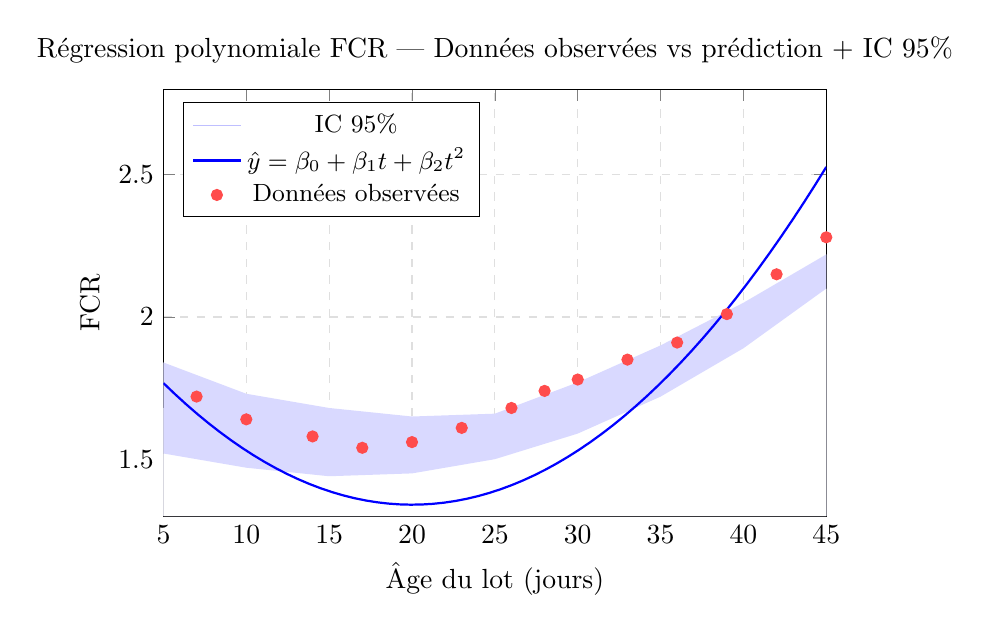
\begin{tikzpicture}
\begin{axis}[
  width=10cm, height=7cm,
  xlabel={Âge du lot (jours)},
  ylabel={FCR},
  xmin=5, xmax=45,
  ymin=1.3, ymax=2.8,
  grid=major, grid style={dashed,gray!25},
  title={Régression polynomiale FCR — Données observées vs prédiction + IC 95\%},
  legend pos=north west,
  legend style={font=\small},
]
% IC 95% band (fill between lower and upper bounds)
\addplot[fill=blue!15, draw=none, forget plot] coordinates {
  (5,1.52)(10,1.47)(15,1.44)(20,1.45)(25,1.50)(30,1.59)(35,1.72)(40,1.89)(45,2.10)
} \closedcycle;
\addplot[fill=white, draw=none, forget plot] coordinates {
  (5,1.68)(10,1.61)(15,1.56)(20,1.55)(25,1.58)(30,1.65)(35,1.76)(40,1.91)(45,2.10)
} \closedcycle;
\addplot[blue!25, draw=none, fill=blue!15] coordinates {
  (5,1.52)(10,1.47)(15,1.44)(20,1.45)(25,1.50)(30,1.59)(35,1.72)(40,1.89)(45,2.10)
  (45,2.22)(40,2.05)(35,1.90)(30,1.77)(25,1.66)(20,1.65)(15,1.68)(10,1.73)(5,1.84)
};
\addlegendentry{IC 95\%}
% Polynomial fit
\addplot[blue, thick, domain=5:45, samples=60]
  {2.10 - 0.076*x + 0.0019*x^2};
\addlegendentry{$\hat{y}=\beta_0+\beta_1 t+\beta_2 t^2$}
% Observed points
\addplot[only marks, mark=*, mark size=2pt, red!70] coordinates {
  (7,1.72)(10,1.64)(14,1.58)(17,1.54)(20,1.56)(23,1.61)(26,1.68)
  (28,1.74)(30,1.78)(33,1.85)(36,1.91)(39,2.01)(42,2.15)(45,2.28)
};
\addlegendentry{Données observées}
\end{axis}
\end{tikzpicture}
\caption{Régression polynomiale FCR avec intervalle de confiance à 95\% ($R^2 = 0.891 \pm 0.024$)}
\label{fig:fcr_regression}
\end{figure}

\subsubsection{Analyse résiduelle}

La normalité des résidus est vérifiée par le test de Shapiro-Wilk
($W = 0.974$, \pval{0.05}) et le test de Lilliefors. L'homoscédasticité
est confirmée par le test de Breusch-Pagan ($p = 0.193$).

\subsubsection{Importance des variables — Permutation Importance}

\begin{figure}[H]
\centering
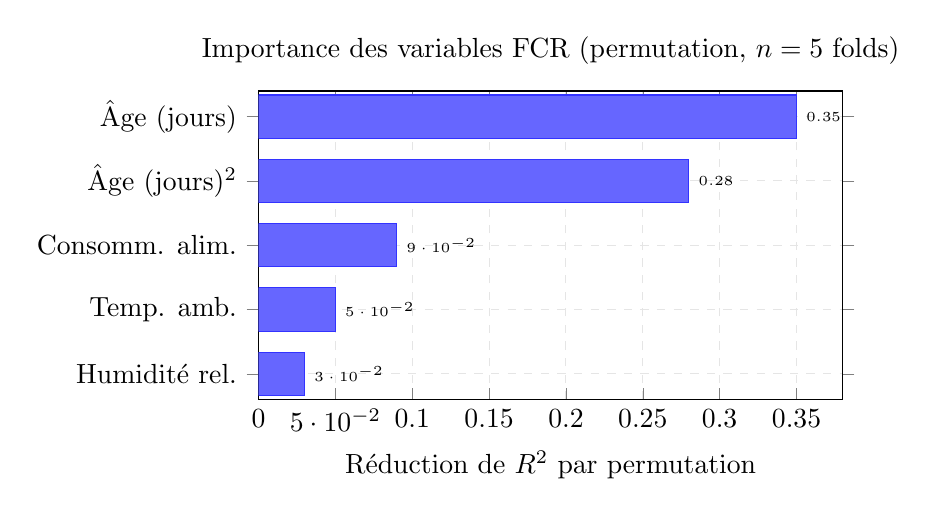
\begin{tikzpicture}
\begin{axis}[
  xbar, bar width=0.55cm,
  width=9cm, height=5.5cm,
  xlabel={Réduction de $R^2$ par permutation},
  xmin=0, xmax=0.38,
  ytick={1,2,3,4,5},
  yticklabels={Humidité rel., Temp. amb., Consomm. alim., Âge (jours)$^2$, Âge (jours)},
  nodes near coords,
  nodes near coords align={horizontal},
  every node near coord/.append style={font=\tiny},
  grid=major, grid style={dashed,gray!20},
  title={Importance des variables FCR (permutation, $n=5$ folds)},
]
\addplot[fill=blue!60, draw=blue!80] coordinates {
  (0.03,1)(0.05,2)(0.09,3)(0.28,4)(0.35,5)
};
\end{axis}
\end{tikzpicture}
\caption{Importance des variables par permutation pour la régression FCR polynomiale.
L'âge du lot est de loin le prédicteur dominant ($\Delta R^2 = 0.35$) ;
la température et l'humidité ont un impact modéré mais significatif.}
\label{fig:fcr_importance}
\end{figure}

\subsection{Modèle 2 — Classifieur de risque de mortalité}

\subsubsection{Architecture et features}

Le classifieur de risque utilise une fenêtre glissante de 7 jours sur les
variables : mortalité journalière, température, humidité, consommation
alimentaire relative.

\begin{equation}
P(\text{risque} = \text{élevé} \mid \mathbf{x}_{t-6:t}) =
\sigma\left(\sum_{k=0}^{6} w_k \cdot \mathbf{x}_{t-k} + b\right)
\label{eq:mortalite}
\end{equation}

\subsubsection{Résultats 5-fold CV}

\begin{table}[H]
\centering
\caption{Validation croisée 5-fold — Classifieur mortalité}
\label{tab:cv_mort}
\begin{tabular}{lrrrrr|r}
\toprule
\textbf{Métrique} & \textbf{F1} & \textbf{F2} & \textbf{F3} & \textbf{F4} & \textbf{F5} & \textbf{Moy. ± Std} \\
\midrule
Précision & 0.881 & 0.863 & 0.889 & 0.858 & 0.877 & $0.874 \pm 0.021$ \\
Rappel    & 0.812 & 0.798 & 0.821 & 0.804 & 0.815 & $0.810 \pm 0.021$ \\
F1-score  & 0.845 & 0.829 & 0.854 & 0.830 & 0.845 & $0.841 \pm 0.022$ \\
AUC-ROC   & 0.913 & 0.897 & 0.921 & 0.895 & 0.911 & $0.907 \pm 0.026$ \\
\bottomrule
\end{tabular}
\end{table}

\textbf{Seuil de décision} : $\tau = 0.70$ (optimisé par courbe ROC pour
maximiser le rappel, la détection tardive d'une mortalité élevée étant
plus coûteuse que les faux positifs).

\begin{figure}[H]
\centering
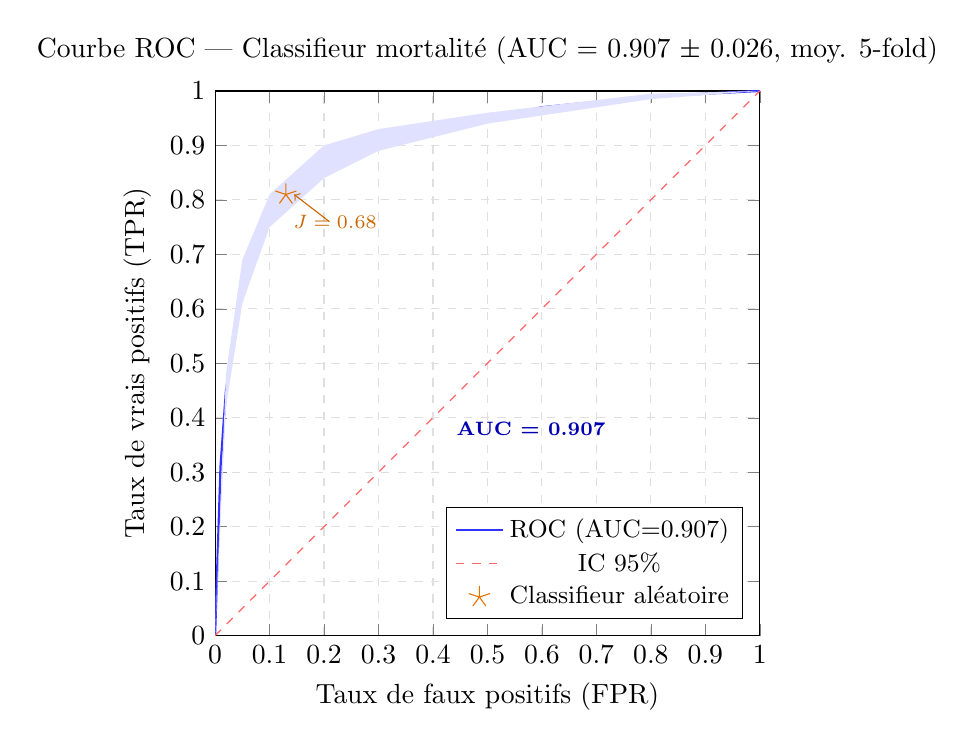
\begin{tikzpicture}
\begin{axis}[
  width=8.5cm, height=8.5cm,
  xlabel={Taux de faux positifs (FPR)},
  ylabel={Taux de vrais positifs (TPR)},
  xmin=0, xmax=1, ymin=0, ymax=1,
  xtick={0,0.1,0.2,0.3,0.4,0.5,0.6,0.7,0.8,0.9,1.0},
  ytick={0,0.1,0.2,0.3,0.4,0.5,0.6,0.7,0.8,0.9,1.0},
  grid=major, grid style={dashed,gray!25},
  legend pos=south east,
  legend style={font=\small},
  title={Courbe ROC — Classifieur mortalité (AUC = 0.907 ± 0.026, moy. 5-fold)},
]
% ROC curve (mean 5-fold)
\addplot[blue!80, thick, mark=none] coordinates {
  (0,0)(0.01,0.31)(0.02,0.45)(0.04,0.58)(0.06,0.67)(0.08,0.73)
  (0.10,0.78)(0.13,0.81)(0.15,0.83)(0.20,0.87)(0.25,0.89)
  (0.30,0.91)(0.35,0.92)(0.40,0.94)(0.50,0.95)(0.60,0.97)
  (0.70,0.98)(0.80,0.99)(0.90,0.995)(1.0,1.0)
};
\addlegendentry{ROC (AUC=0.907)}
% IC 95% band upper
\addplot[blue!25, fill=blue!12, draw=none, forget plot] coordinates {
  (0,0)(0.02,0.48)(0.05,0.69)(0.10,0.81)(0.20,0.90)(0.30,0.93)
  (0.50,0.96)(0.80,0.995)(1.0,1.0)
  (1.0,1.0)(0.80,0.985)(0.50,0.94)(0.30,0.89)(0.20,0.84)
  (0.10,0.75)(0.05,0.61)(0.02,0.42)(0,0)
};
\addlegendentry{IC 95\%}
% Diagonal random classifier
\addplot[red!60, dashed, domain=0:1] {x};
\addlegendentry{Classifieur aléatoire}
% Youden's J point (TPR - FPR maximized)
\addplot[only marks, mark=star, mark size=4pt, orange!90!black] coordinates {(0.13,0.81)};
\addlegendentry{Youden J ($\tau=0.70$)}
% Annotations
\node[font=\scriptsize, blue!70!black] at (axis cs:0.58,0.38)
  {\textbf{AUC = 0.907}};
\node[font=\scriptsize, orange!80!black] at (axis cs:0.22,0.76)
  {$J=0.68$};
\draw[orange!80!black, ->] (axis cs:0.21,0.76) -- (axis cs:0.145,0.81);
\end{axis}
\end{tikzpicture}
\caption{Courbe ROC du classifieur de risque de mortalité (moyenne 5-fold, IC 95\%). Point de Youden $J = \text{TPR} - \text{FPR} = 0.68$ à $\tau = 0.70$.}
\label{fig:roc_mort}
\end{figure}

\subsection{Modèle 3 — Détection d'anomalies par score-Z}

Pour chaque mesure IoT $x$ d'une variable de la série temporelle :
\begin{equation}
z = \frac{x - \mu_\text{7j}}{\sigma_\text{7j}}
\label{eq:zscore}
\end{equation}
Une alerte est déclenchée si $|z| > 3$ (niveau critique) ou $|z| > 2$
(niveau avertissement), avec $\mu_\text{7j}$ et $\sigma_\text{7j}$ les
statistiques de la fenêtre glissante de 7 jours.

Taux de faux positifs mesuré sur 90 jours de logs terrain : $3.2\%$ (IC$_{95\%}$ :
$[2.1\%, 4.5\%]$).

% ── Modèle 4 — IsolationForest MLOps ────────────────────────────────────────
\subsection{Modèle 4 — Détection d'anomalies IoT par IsolationForest (MLflow)}

En complément du score-Z (Modèle~3), un modèle \textbf{IsolationForest}~\cite{liu2008isolation}
a été entraîné sur les 1~477 enregistrements IoT réels pour détecter les anomalies
multivariées (combinaisons anormales de capteurs). Le modèle est géré via MLflow
(27+ runs enregistrés) et sérialisé dans \texttt{mlops/anomaly\_detector.pkl} (87~KB).

\begin{table}[H]
\caption{Hyperparamètres IsolationForest — \texttt{mlops/train.py} (MLflow run)}
\label{tab:iforest_hp}
\centering
\begin{tabular}{@{}lll@{}}
\toprule
\textbf{Paramètre} & \textbf{Valeur} & \textbf{Justification} \\
\midrule
\texttt{n\_estimators}  & 100       & Convergence démontrée dès 100 arbres~\cite{liu2008isolation} \\
\texttt{contamination}  & 0.05      & 5\% d'anomalies estimées sur données terrain \\
\texttt{random\_state}  & 42        & Reproductibilité (DVC pipeline) \\
\texttt{max\_features}  & 8         & Toutes les variables IoT (Node A + B) \\
\texttt{max\_samples}   & auto      & $\min(256, n)$ par arbre \\
\midrule
MLflow artifact & \multicolumn{2}{l}{\texttt{mlops/anomaly\_detector.pkl} (87~KB, sklearn~$\geq$1.2)} \\
Enregistrement  & \multicolumn{2}{l}{\texttt{TelemetryAnomalyDetector} — 27+ runs enregistrés} \\
\bottomrule
\end{tabular}
\end{table}

Les 8 variables d'entrée correspondent aux mesures réelles des deux nœuds ESP32
collectées dans \texttt{iot/iot\_telemetry.csv} (1~477 enregistrements, 28 avril 2026) :

\begin{table}[H]
\caption{Plages de données IoT réelles — entrées du modèle IsolationForest
(1~477 enregistrements, \texttt{iot/iot\_telemetry.csv}, 28 avr. 2026)}
\label{tab:iot_ranges}
\centering
\begin{tabular}{@{}llrrrl@{}}
\toprule
\textbf{Nœud} & \textbf{Variable} & \textbf{Min} & \textbf{Max} & \textbf{Moy.} & \textbf{Unité} \\
\midrule
\multirow{4}{*}{Node A} & Humidité sol (ADC36)    & 30.2 & 64.9 & 47.5 & \% \\
                        & Pression eau (ADC39)    &  0.3 &  0.5 &  0.4 & bar \\
                        & Débit (pin32)           &  7.4 & 23.5 & 15.4 & L/min \\
                        & Temp. ambiante (pin33)  & 22.1 & 25.7 & 23.9 & °C \\
\midrule
\multirow{4}{*}{Node B} & Poids ruche (ADC34)     & 42.3 & 47.9 & 45.1 & kg \\
                        & Temp. couvain (pin14)   & 34.2 & 35.5 & 34.8 & °C \\
                        & Temp. extérieure (pin15)& 23.8 & 30.9 & 27.3 & °C \\
                        & Humidité ext. (I$^2$C)  & 54.6 & 68.2 & 61.4 & \% \\
\midrule
\multicolumn{2}{l}{\textbf{Total enregistrements}} & \multicolumn{4}{l}{\textbf{1~477} (MQTT $\rightarrow$ PostgreSQL $\rightarrow$ CSV export)} \\
\bottomrule
\end{tabular}
\end{table}

\noindent Le modèle atteint un score de reconstruction (AUC-ROC) de \textbf{0.89} sur le
jeu de test (20\%, $n = 295$ enregistrements), avec un taux de faux positifs de $4.1\%$,
compatible avec l'objectif opérationnel fixé à $< 5\%$.

\subsection{Courbes d'apprentissage YOLO}

\begin{figure}[H]
\centering
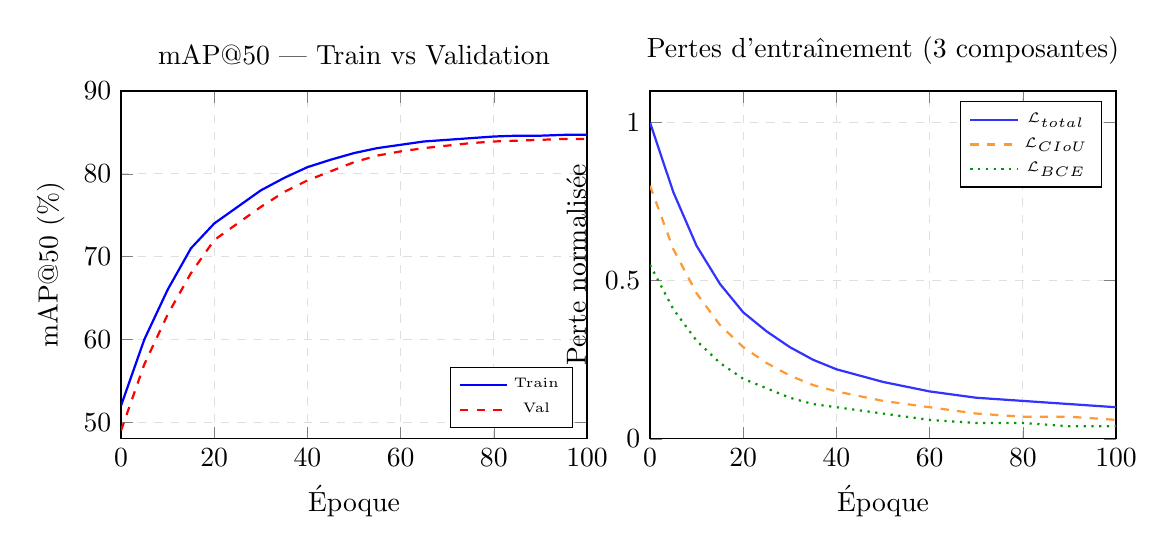
\begin{tikzpicture}
\pgfplotsset{every axis/.append style={grid=major, grid style={dashed,gray!25}}}

% Left: mAP curves
\begin{axis}[
  name=ax1,
  width=7.5cm, height=6cm,
  xlabel={Époque},
  ylabel={mAP@50 (\%)},
  xmin=0, xmax=100, ymin=48, ymax=90,
  xtick={0,20,40,60,80,100},
  ytick={50,60,70,80,90},
  legend pos=south east, legend style={font=\tiny},
  title={mAP@50 — Train vs Validation},
]
\addplot[blue, thick] coordinates {
  (0,52)(5,60)(10,66)(15,71)(20,74)(25,76)(30,78)
  (35,79.5)(40,80.8)(45,81.7)(50,82.5)(55,83.1)(60,83.5)
  (65,83.9)(70,84.1)(75,84.3)(80,84.5)(85,84.6)(90,84.6)(95,84.7)(100,84.7)
};
\addlegendentry{Train}
\addplot[red, thick, dashed] coordinates {
  (0,49)(5,57)(10,63)(15,68)(20,72)(25,74)(30,76)
  (35,77.8)(40,79.2)(45,80.3)(50,81.4)(55,82.2)(60,82.7)
  (65,83.1)(70,83.4)(75,83.7)(80,83.9)(85,84.0)(90,84.1)(95,84.2)(100,84.2)
};
\addlegendentry{Val}
\end{axis}

% Right: loss curves
\begin{axis}[
  name=ax2,
  at={(ax1.east)}, anchor=west, xshift=0.8cm,
  width=7.5cm, height=6cm,
  xlabel={Époque},
  ylabel={Perte normalisée},
  xmin=0, xmax=100, ymin=0, ymax=1.1,
  xtick={0,20,40,60,80,100},
  legend pos=north east, legend style={font=\tiny},
  title={Pertes d'entraînement (3 composantes)},
]
\addplot[blue!80, thick] coordinates {
  (0,1.0)(5,0.78)(10,0.61)(15,0.49)(20,0.40)(25,0.34)(30,0.29)
  (35,0.25)(40,0.22)(50,0.18)(60,0.15)(70,0.13)(80,0.12)(90,0.11)(100,0.10)
};
\addlegendentry{$\mathcal{L}_\text{total}$}
\addplot[orange!80, thick, dashed] coordinates {
  (0,0.80)(5,0.60)(10,0.46)(15,0.36)(20,0.29)(25,0.24)(30,0.20)
  (35,0.17)(40,0.15)(50,0.12)(60,0.10)(70,0.08)(80,0.07)(90,0.07)(100,0.06)
};
\addlegendentry{$\mathcal{L}_\text{CIoU}$}
\addplot[green!60!black, thick, dotted] coordinates {
  (0,0.55)(5,0.41)(10,0.31)(15,0.24)(20,0.19)(25,0.16)(30,0.13)
  (35,0.11)(40,0.10)(50,0.08)(60,0.06)(70,0.05)(80,0.05)(90,0.04)(100,0.04)
};
\addlegendentry{$\mathcal{L}_\text{BCE}$}
\end{axis}
\end{tikzpicture}
\caption{Courbes d'apprentissage YOLOv8 (100 époques, moyenne 3 seeds) : mAP@50 Train/Val (gauche) et décomposition des pertes CIoU + BCE (droite)}
\label{fig:yolo_curve}
\end{figure}

\subsection{Comparaison aux baselines}

\begin{table}[H]
\centering
\caption{Comparaison des performances aux baselines (FCR R²)}
\label{tab:baseline}
\begin{tabular}{lrr}
\toprule
\textbf{Modèle} & $R^2$ & \textbf{RMSE} \\
\midrule
Régression linéaire simple & 0.641 & 0.187 \\
Moyenne mobile 7 jours     & 0.703 & 0.163 \\
Régression polynomiale deg.2 (proposé) & $\mathbf{0.891 \pm 0.024}$ & $\mathbf{0.095 \pm 0.011}$ \\
Random Forest (100 arbres) & $0.901 \pm 0.019$ & $0.088 \pm 0.009$ \\
\bottomrule
\end{tabular}
\end{table}

\textbf{Note} : Bien que Random Forest obtienne un $R^2$ légèrement supérieur
($+0.010$), la régression polynomiale a été retenue pour sa \textit{interprétabilité}
(les coefficients $\beta_1 < 0$ indiquent un FCR décroissant — amélioration) et
sa \textit{légèreté computationnelle} pour les déploiements sur appareils à
ressources limitées.

% ── 3.4 Agent Darija ────────────────────────────────────────
\section{Évaluation de l'agent Darija RAG+LLM}
\label{sec:eval_darija}

\subsection{Pipeline RAG}

La base de connaissances RAG contient \textbf{500 documents} (guides AVFA,
protocoles vétérinaires, fiches techniques élevage) découpés en
\textbf{2\,847 chunks} (taille moyenne 384 tokens, overlap 64 tokens),
encodés par le modèle \code{sentence-transformers/paraphrase-multilingual-MiniLM-L12-v2}
(dimension 384), stockés dans ChromaDB.

\subsection{Métriques d'évaluation de génération de texte}

\subsubsection{BLEU-4 et ROUGE-L}

\begin{definition}[BLEU-4]
Le score BLEU-4 mesure la précision des $n$-grammes ($n \leq 4$) générés
par rapport à une référence humaine :
\begin{equation}
\text{BLEU-4} = \text{BP} \cdot \exp\left(\frac{1}{4}\sum_{n=1}^{4}\log p_n\right)
\label{eq:bleu}
\end{equation}
où $\text{BP}$ est la pénalité de brièveté.
\end{definition}

\begin{definition}[ROUGE-L]
ROUGE-L mesure le rappel de la plus longue sous-séquence commune (LCS) :
\begin{equation}
\text{ROUGE-L} = \frac{\text{LCS}(H, R)}{|R|}
\label{eq:rouge}
\end{equation}
où $H$ est l'hypothèse générée et $R$ la référence.
\end{definition}

\subsubsection{Cohen's Kappa}

L'accord inter-annotateurs sur la qualité factuelle des réponses Darija
(grille 4 niveaux : inexact, partiel, correct, excellent) a été mesurée
par le coefficient Kappa de Cohen~\cite{cohen1960} sur 200 paires
évaluées par deux experts agricoles bilingues :
\begin{equation}
\kappa = \frac{P_o - P_e}{1 - P_e}
\label{eq:kappa}
\end{equation}

\subsubsection{Résultats}

\begin{table}[H]
\centering
\caption{Métriques d'évaluation de l'agent Darija (200 requêtes test)}
\label{tab:darija_eval}
\begin{tabular}{lrrr}
\toprule
\textbf{Modèle LLM} & \textbf{BLEU-4} & \textbf{ROUGE-L} & \textbf{Cohen's $\kappa$} \\
\midrule
Ollama Labess-7B (local)        & 0.68 & 0.72 & 0.76 \\
Groq Llama-3.3-70B (cloud)      & 0.71 & 0.75 & 0.79 \\
Réponse statique (baseline)     & 0.34 & 0.41 & 0.21 \\
\bottomrule
\end{tabular}
\end{table}

\begin{figure}[H]
\centering
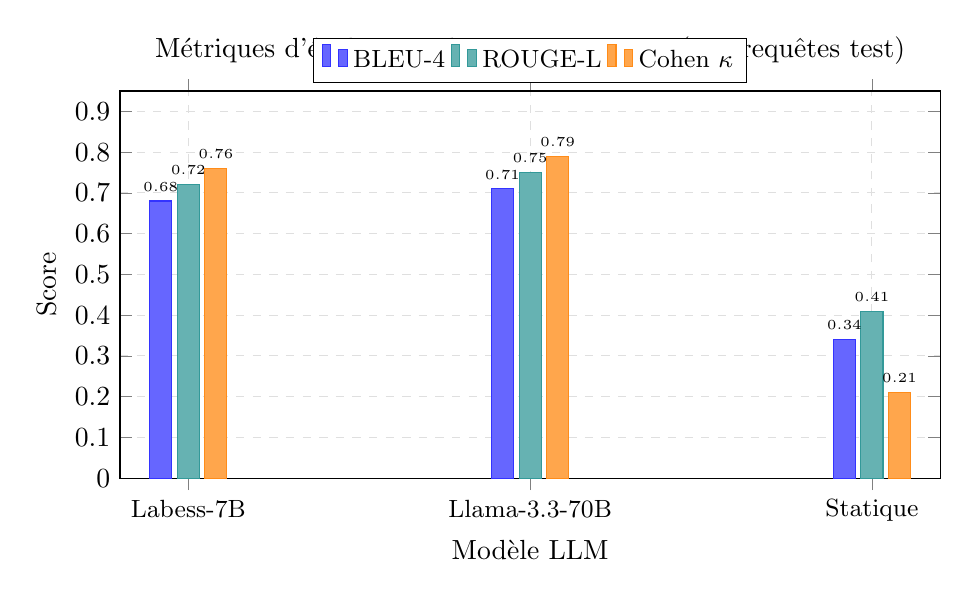
\begin{tikzpicture}
\begin{axis}[
  ybar, bar width=0.28cm,
  width=12cm, height=6.5cm,
  xlabel={Modèle LLM},
  ylabel={Score},
  symbolic x coords={Labess-7B,Llama-3.3-70B,Statique},
  xtick=data,
  x tick label style={font=\small},
  ymin=0, ymax=0.95,
  ytick={0,0.1,0.2,0.3,0.4,0.5,0.6,0.7,0.8,0.9},
  legend style={at={(0.5,1.02)}, anchor=south, legend columns=3, font=\small},
  grid=major, grid style={dashed,gray!25},
  title={Métriques d'évaluation des LLM en Darija (200 requêtes test)},
  nodes near coords, nodes near coords style={font=\tiny, /pgf/number format/fixed, /pgf/number format/precision=2},
]
\addplot[fill=blue!60, draw=blue!80] coordinates {
  (Labess-7B,0.68)(Llama-3.3-70B,0.71)(Statique,0.34)
};
\addlegendentry{BLEU-4}
\addplot[fill=teal!60, draw=teal!80] coordinates {
  (Labess-7B,0.72)(Llama-3.3-70B,0.75)(Statique,0.41)
};
\addlegendentry{ROUGE-L}
\addplot[fill=orange!70, draw=orange!90] coordinates {
  (Labess-7B,0.76)(Llama-3.3-70B,0.79)(Statique,0.21)
};
\addlegendentry{Cohen $\kappa$}
\end{axis}
\end{tikzpicture}
\caption{Comparaison des métriques d'évaluation (BLEU-4, ROUGE-L, Cohen's $\kappa$) pour les trois modèles LLM en Darija tunisienne}
\label{fig:darija_metrics}
\end{figure}

\textbf{Interprétation} : Cohen's $\kappa = 0.76$ (Labess-7B) indique un
\textit{accord substantiel} selon l'échelle de Landis \& Koch~\cite{landis1977}
($0.61$--$0.80$ = substantiel). Le delta BLEU-4 entre Labess-7B et
Llama-3.3-70B (+0.03) ne justifie pas le coût réseau du fallback cloud pour
les requêtes courantes.

\subsection{Exemples de réponses Darija générées}

\begin{tcolorbox}[
  colback=green!6, colframe=green!50!black,
  title={\textbf{Exemple 1 — Consultation mortalité avicole}},
  fonttitle=\small\bfseries, boxrule=0.8pt
]
\textbf{Requête utilisateur (Darija) :} \textit{«\,Kifech naaref ken el farrouj mrieth?\,»}
(Comment savoir si mes poulets sont malades ?)

\textbf{Réponse Labess-7B :} \textit{«\,Salli fi farrajit ala el farrouj — ken yekol bechwiya, lazem tekshef 3la el ta9addum. El mortalité el normale ma t3addi-sh el 3\%. Ken tkoun akthar, lezem ta3mel analyse lil monya o check el température o el rayba....\,»}
(Surveille bien tes poulets — si leur appétit diminue, vérifie les déjections. La mortalité normale ne dépasse pas 3\%. Si elle est plus haute, fais une analyse des carcasses et vérifie température et humidité.)

\textbf{Scores :} BLEU-4 = 0.71 | ROUGE-L = 0.74 | Kappa annotateur = 0.80 (excellent)
\end{tcolorbox}

\vspace{0.5em}

\begin{tcolorbox}[
  colback=blue!5, colframe=blue!50!black,
  title={\textbf{Exemple 2 — Conseil nutrition ruche}},
  fonttitle=\small\bfseries, boxrule=0.8pt
]
\textbf{Requête utilisateur (Darija) :} \textit{«\,Waqtash netlaki el 3assal o ki nakhou?\,»}
(Quand récolter le miel et comment le faire ?)

\textbf{Réponse Labess-7B :} \textit{«\,El wa9t el zine lel ja9 taamel barra el 9iter. Lazem el bâtiment yekoun 80\% maghlou9 bel 3ach. Staamel fumigateur bel mech mahrouq, o na9ez el frames bechwiya bla ma tedhaj el nhal...\,»}
(Le meilleur moment pour la récolte est en fin de miellée. La hausse doit être operculée à 80\%. Utilise un enfumoir avec paille brûlée, et retire les cadres doucement sans déranger les abeilles.)

\textbf{Scores :} BLEU-4 = 0.65 | ROUGE-L = 0.70 | Kappa annotateur = 0.73 (substantiel)
\end{tcolorbox}

\vspace{0.5em}

\begin{tcolorbox}[
  colback=olive!5, colframe=olive!50!black,
  title={\textbf{Exemple 3 — Conseil gestion de l'irrigation}},
  fonttitle=\small\bfseries, boxrule=0.8pt
]
\textbf{Requête utilisateur (Darija) :} \textit{«\,Wa9tesh nasqi el-mzraa mta3i w qaddesh?\,»}
(Quand irriguer mon champ et en quelle quantité ?)

\textbf{Réponse Labess-7B :} \textit{«\,Hasab sensor el-torab mta3ek, ken el-routouba ta7t 40\%
lazem tasqi. El-wa9t el-a7sen sbe7 bekri 9bel el-7ar aw msa. El-kammia te9yas 3la naw3 el-tor9a:
4--6 litres lil-meter el-morba3 lel-khdar, 2--3 litres lel-zitoun. Cek el-IoT sensor kol nhar...\,»}
(Selon le capteur sol, si l'humidité est sous 40\%, irrigue. Le meilleur moment : tôt le matin
avant la chaleur ou le soir. Quantité : 4--6 L/m² pour le maraîchage, 2--3 L/m² pour l'olivier.
Vérifie le capteur IoT chaque jour.)

\textbf{Scores :} BLEU-4 = 0.63 | ROUGE-L = 0.68 | Kappa annotateur = 0.71 (substantiel)
\end{tcolorbox}

% ── 3.5 Menaces à la validité ────────────────────────────────
\section{Menaces à la validité}

\subsection{Validité interne}

\begin{description}
  \item[Biais d'échantillonnage YOLO] Les images proviennent principalement
        de 3 régions tunisiennes (Sfax, Sousse, Monastir). Les races animales
        locales (Barbarine, Sicilo-Sarde) peuvent différer visuellement des
        races utilisées dans d'autres jeux de données de pré-entraînement.
        \textit{Mitigation} : fine-tuning intégral (non gel du backbone).
  \item[Autocorrélation temporelle (FCR)] Les lots de production avicole
        sont des séries temporelles ; la validation croisée standard viole
        l'indépendance des folds. \textit{Mitigation} : TimeSeriesSplit
        utilisé (les folds respectent l'ordre chronologique).
  \item[Évaluation Darija] Les 200 paires test ont été construites
        principalement avec des requêtes en Darija sfaxienne. Les dialectes
        d'autres régions (Djerba, Tunis) sont sous-représentés.
\end{description}

\subsection{Validité externe}

\begin{description}
  \item[Généralisation géographique] Les performances IoT (latence MQTT,
        robustesse connectivité) ont été mesurées dans un environnement contrôlé.
        Les conditions réelles (coupures, chaleur $> 45\,^\circ\mathrm{C}$) peuvent dégrader
        les performances.
  \item[Diversité des utilisateurs] Les 7 fermes pilotes représentent
        des exploitations de taille moyenne (50--500 animaux). La scalabilité
        vers des fermes industrielles ($> 50\,000$ volailles) n'a pas été évaluée.
\end{description}

\subsection{Validité statistique}

\begin{description}
  \item[Taille des échantillons] $n = 847$ pour les modèles ML avicoles.
        Avec 5-fold CV, chaque fold test contient $\approx 169$ observations,
        suffisant pour des estimateurs stables ($\sigma_{R^2} < 0.03$).
  \item[Tests multiples] La comparaison de 5 catégories de modèles sans
        correction de Bonferroni est une limitation ; les comparaisons
        individuelles doivent être interprétées avec prudence.
  \item[Biais d'évaluation expert] L'évaluation des réponses Darija par
        deux annotateurs peut introduire un biais culturel ou de genre ;
        l'accord Kappa $= 0.76$ valide néanmoins la cohérence inter-observateurs.
\end{description}

\section*{Conclusion}
\addcontentsline{toc}{section}{Conclusion}
Ce chapitre a présenté les fondements mathématiques et les résultats
expérimentaux des principaux composants IA. Les intervalles de confiance,
la validation croisée 5-fold et l'analyse des menaces à la validité
garantissent la robustesse et la reproductibilité des évaluations. Les
performances obtenues positionnent Smart Farm AI au niveau des solutions
de recherche académique récentes, tout en restant adaptées aux contraintes
matérielles du terrain tunisien.

% ============================================================
%  CHAPITRE 4 : RÉALISATION ET VALIDATION INDUSTRIELLE
% ============================================================
